\documentclass{article}
% To modify the size of the page:
\usepackage[dvips,a0paper,landscape,centering,left=5cm,right=5cm,top=5cm, bottom=5cm]{geometry}
\usepackage[english, serbian c]{babel}
\usepackage{multicol}
\usepackage[utf8]{inputenc}
\usepackage{color,xcolor}
\usepackage{float}
\usepackage{amsmath, amsthm, amsfonts}
\usepackage{graphicx}           % Include figure files.
\usepackage{anyfontsize}
\usepackage{setspace}
\usepackage{lipsum}
% Colors
% -------
\usepackage[immediate]{silence}
\WarningFilter[temp]{latex}{Command} % silence the warning
\definecolor{azulcielo}{RGB}{227,243,248}

\newcommand\Mark[1]{\textsuperscript#1}
\pagestyle{empty}

\def\to{\rightarrow}
\usepackage{geometry}
\usepackage{layout}
\usepackage{url}
\usepackage[pdftex, pdfborderstyle={/S/U/W 0}]{hyperref}
\usepackage{csquotes}
\usepackage[backend=biber, style=ieee,language=auto]{biblatex}
\addbibresource{bibliography.bib}

\graphicspath{{media/images/}}
\DeclareGraphicsExtensions{.jpeg,.png,.jpg}
\usepackage{sectsty}
\sectionfont{\fontsize{60}{72}\selectfont}

% ===========================================================================

\title{}
\author{}
\date{}

\begin{document}
%\maketitle

\begin{center}
  \begin{minipage}{.16\linewidth}
  \qquad\qquad
    
\includegraphics[width=.7\linewidth]{media/images/grb.png}
    ~\vfill
    ~\vfill
  \end{minipage}
  %&
  \begin{minipage}{.6\linewidth}
    \begin{center}
       \textsf{\textbf{{\fontsize{90}{108}\selectfont Дигиталне урбане мреже и друштвени медији}}}\\\vspace{1cm}
       \textrm{\fontsize{40}{48}\selectfont Тамара Јевтимијевић, 261/2017 \\\vspace{5mm} \textit{Рачунарство и друштво}, \textit{Математички факултет у Београду}\\\vspace{10mm} Email: mi17261@alas.matf.bg.ac.rs}  
    \end{center}
  \end{minipage}
  %&
  \hspace{.03\linewidth}
    \begin{minipage}{.16\linewidth}
  \qquad\qquad
    
\includegraphics[width=.7\linewidth]{media/images/grb.png}
    ~\vfill
    ~\vfill
  \end{minipage}
\end{center}

\vspace{2cm}

% ---------------------------------------------------------------------------
\fontsize{30}{36}\selectfont
\setlength{\columnsep}{1cm}

\vspace{200}
\begin{multicols}{3}
% ---------------------------------------------------------------------------

\noindent
\fcolorbox{black}{azulcielo}{
  \begin{minipage}[H]{.96\linewidth}
    \begin{center}
      \vspace{1cm}
      \section*{}
Крајем двадесетог и почетком двадесет првог века информационо-комуникационе корпорације су доживеле највећу експанзију. Данас их има све више и све су више утицајне. Технологија је узнапредовала великом брзином и своје гране је пустила свуда. Данас где год да се окренемо дигитализација је око нас. У наставку ће бити више речи о томе како је дигитализација допринела развоју градова, побољшању живота људи у градовима и како су технологије заокупирале читав свет.
      \vspace{1cm}
    \end{center}
  \end{minipage}
  
}

\section*{Друштвене мреже и град}
\noindent Успон друштвених мрежа као што су Facebook, Twitter, WeChat, Tumblr, Instagram, Google+, YouTube, Linkedin, TikTok, Snapchat и WhatsApp такође је променио начин на који људи широм света комуницирају и живе. Чини се да људи више воле и примењују дигиталне интеракције у односу на физичке интеракције. 
Процењује се да преко 3,2 милијарде људи широм света користите друштвене мреже на овај или онај начин, а ови трендови су заслужни за широк продор паметних уређаја као што су мобилни телефони и таблети.

\begin{center}
    \vspace{1cm}
    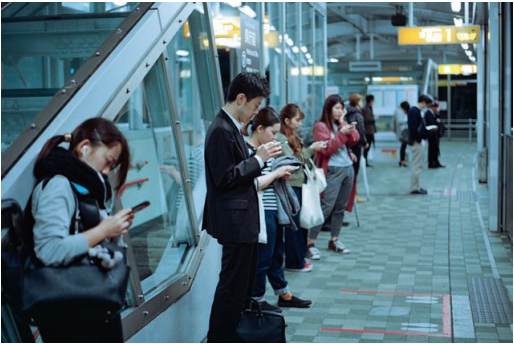
\includegraphics[width=35cm,height=25cm]{media/images/drustvene_mreze.png}
\end{center}
% ---------------------------------------------------------------------------

\section*{Урбано брендирање и друштвене мреже}
\noindent Појава дигиталних решења која се фокусирају на градове и урбана подручја је имала бројне позитивне стране као што је могућност брендирања града. Дигитални бренд је дао градовима прилику да дигиталне технологије искористе на економској граници. Након појаве друштвених мрежа, туристички брендови су прихваћени у различитим градовима кроз стратегије прилагођене различитим корисницима на различитим платформама друштвених мрежа. \\
Брендирање је стратегија која је невино усвојена, да би се они, који живе у неком граду и у њему раде, али и они који су га само посетили осетили његовим делом. 

\begin{center}
    \vspace{1cm}
    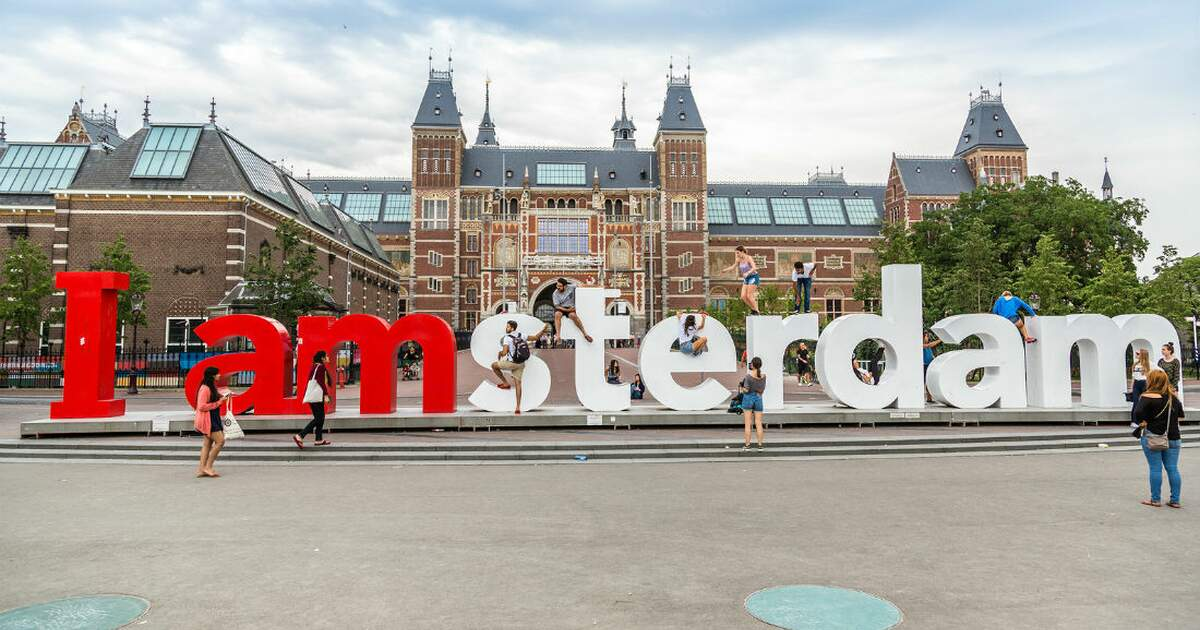
\includegraphics[width=35cm,height=27cm]{media/images/rijksmuseum-amsterdam-museum-iamsterdam.jpg}
\end{center}

% ---------------------------------------------------------------------------
%

\end{multicols}

\end{document}
